\newpage
\section{引言}\zihao{-4}
\setcounter{table}{0}
\setcounter{figure}{0}
\subsection{研究背景}
\par 近年来,人工智能在全球无论是否是计算机相关行业中,都掀起了一股热潮,尤其是深度学习更是赚足了眼球。而GPU现代机器学习应用中计算能力的支撑,在训练、推理、部署等过程中都极大提升了机器学习应用的性能,可以说正是并行高性能计算硬件的发展支撑了深度学习的发展,而英伟达(NVIDIA)更是在并行硬件领域独占鳌头。
\par 在2017年第三季度,英伟达发布了一款基于伏特架构(Volta)的面向深度学习的GPU,Tesla V100\cite{TESLAV100},其中搭载了一些实验性的新技术;之后在2018年第三季度,英伟达发布了新一代图灵架构(Turing),在该架构中,正式引入了许多革命性的新技术,同时也对原有技术做了很大的改进。有面向深度神经网络应用的张量核心(Tensor Core)\cite{TENSORCORE},能够大幅加速在神经网络训练、推理中的混合精度矩阵计算,该核心最先实验性地搭载于Tesla V100,在图灵架构中上至面向深度学习推理的Tesla T4,下至面向游戏玩家的RTX 2080TI都搭载了这款核心;用于更高效搭建分布式计算平台的第二代端对端互联总线(NV Link 2.0)\cite{NVLINK2},相对于原有的QPI等总线,该总线能够直接互连GPU,且提供远高于原先SLI技术所能提供的带宽;以及GPU中计算单元、调度单元、纹理单元等的优化。此外,新架构还针对游戏玩家推出了如实时光线追踪(RTX)、基于深度学习的抗锯齿技术(DLSS)等。
\par 在并行软件方面,与硬件一起,英伟达将其面向并行程序开发的SDK CUDA的版本更新到了10.0,在游戏应用、通用计算方面针对新架构的特性进行了优化;同时发布了基于CUDA 10.0的面向线性代数计算的模板库CUTLASS(CUDA Template Linear Algebra Subroutines)\cite{CUTLASS}以利用其张量核心进行高效的代数运算。
\par 然而,官方文档给出的性能提升仅仅包括单一模块的理论性能提升,如传统CUDA核心的浮点数值计算的理论峰值,新加入的张量核心的混合矩阵计算(GEMM)的理论峰值,NV Link 2.0的理论峰值带宽等。在实际使用中,用户反映在网络推理方面以及基于支持新硬件的相关框架开发的机器学习应用中,提升并没有官方白皮书给出的的9倍之多\cite{VOLTAWHITEPAPER},且同类型不同规模应用的性能提升幅度并不一致,性能提升对神经网络中参数数量、网络层数等因素较为敏感,图 \ref{fig.PerfCompare}为官方白皮书给出的性能提升与实际由Stefano等人评估所得的性能提升的比较,两者存在较大的差距。实际上,官方给出的文档中的提升也仅为绝对计算性能的提升,没有考虑应用类型、平台构建等条件。目前关于新架构GPU的研究主要集中在大型计算节点的扩展效率 \cite{EXASCLEDL},基于GPGPU-SIM模拟的性能考察等\cite{MODELING},这些研究或是停留在表征性能层面、没有深入到代码或是中间代码层面;或是使用模拟技术、在PC机上进行模拟,尽管目前对于硬件的模拟运行的匹配度能够达到较高的水准,但由于版本老旧,仍有一定偏差,目前GPGPU-SIM的稳定版支持的最高的CUDA SDK版本为4.0,开发版本支持的最高的CUDA SDK版本为9.2。本文将直接针对真实的,单一的,图灵架构的GPU:RTX 2080TI进行深入,结合CUDA SDK 10.0以及对应的软件库包含CUTLASS,CUBLAS等,从架构、PTX 中间代码层面、SASS机器码层面对GPU在使用GPU加速的机器学习应用中的性能以及性能提升进行研究和评估;根据研究和评估结果以及分析得到的原因对现有CUDA代码、基于框架的应用源码进行优化。同时根据实验结果提出合理地假设与展望。
\begin{figure}
	\centering
	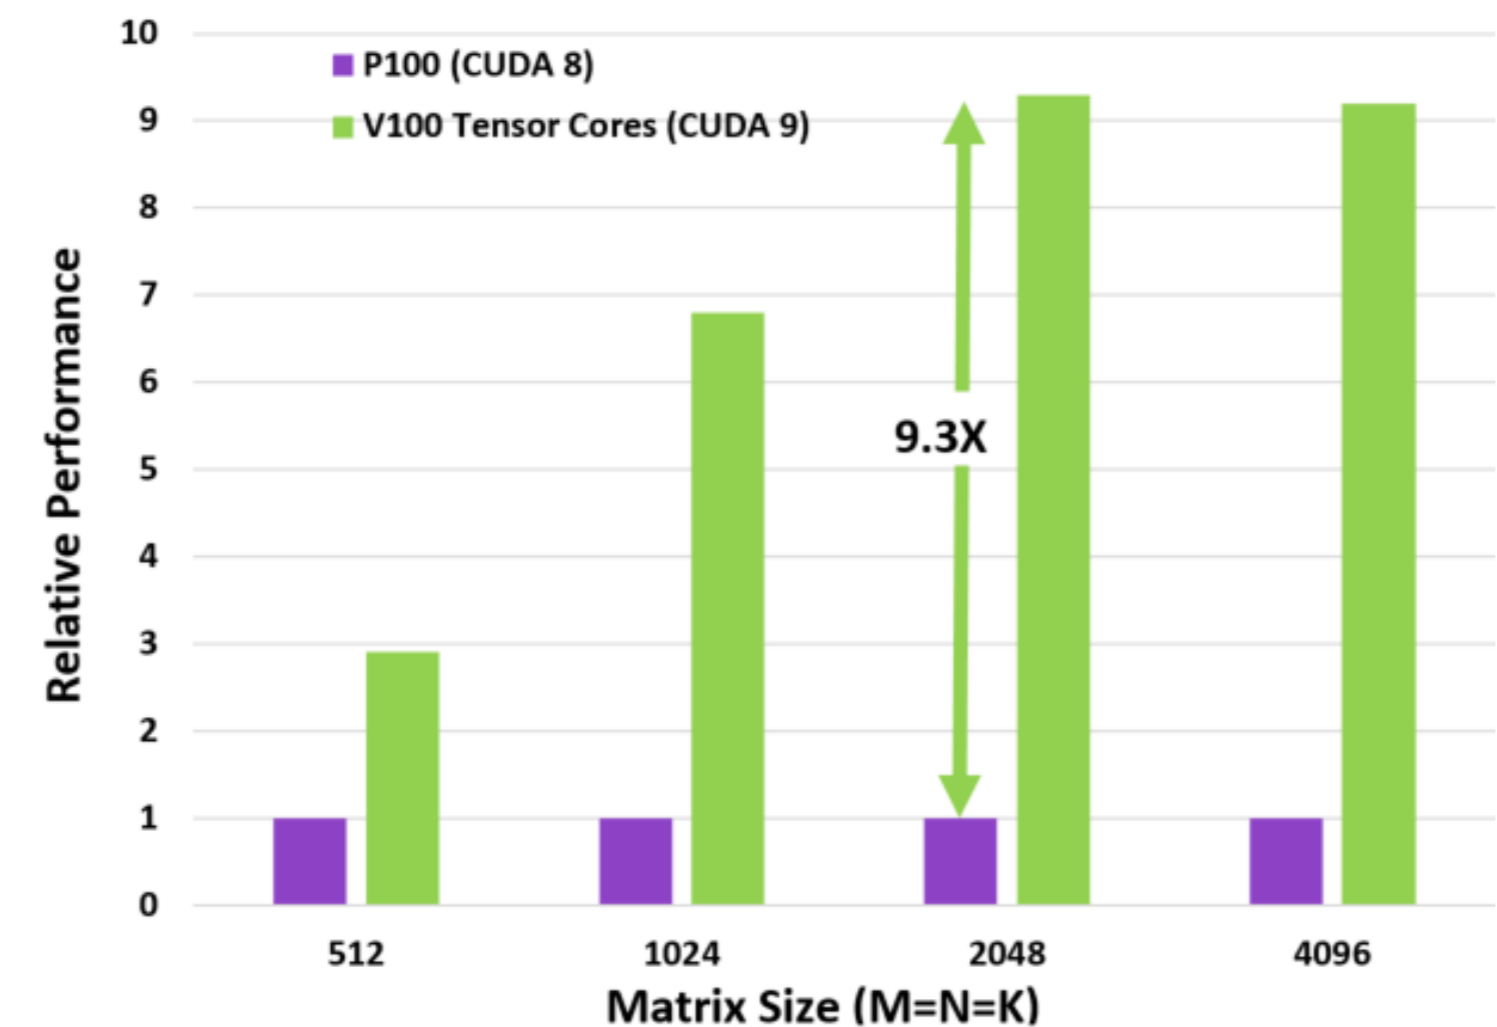
\includegraphics[width=7.5cm,height=5cm]{figures/VoltaGemmPerf.jpg}
	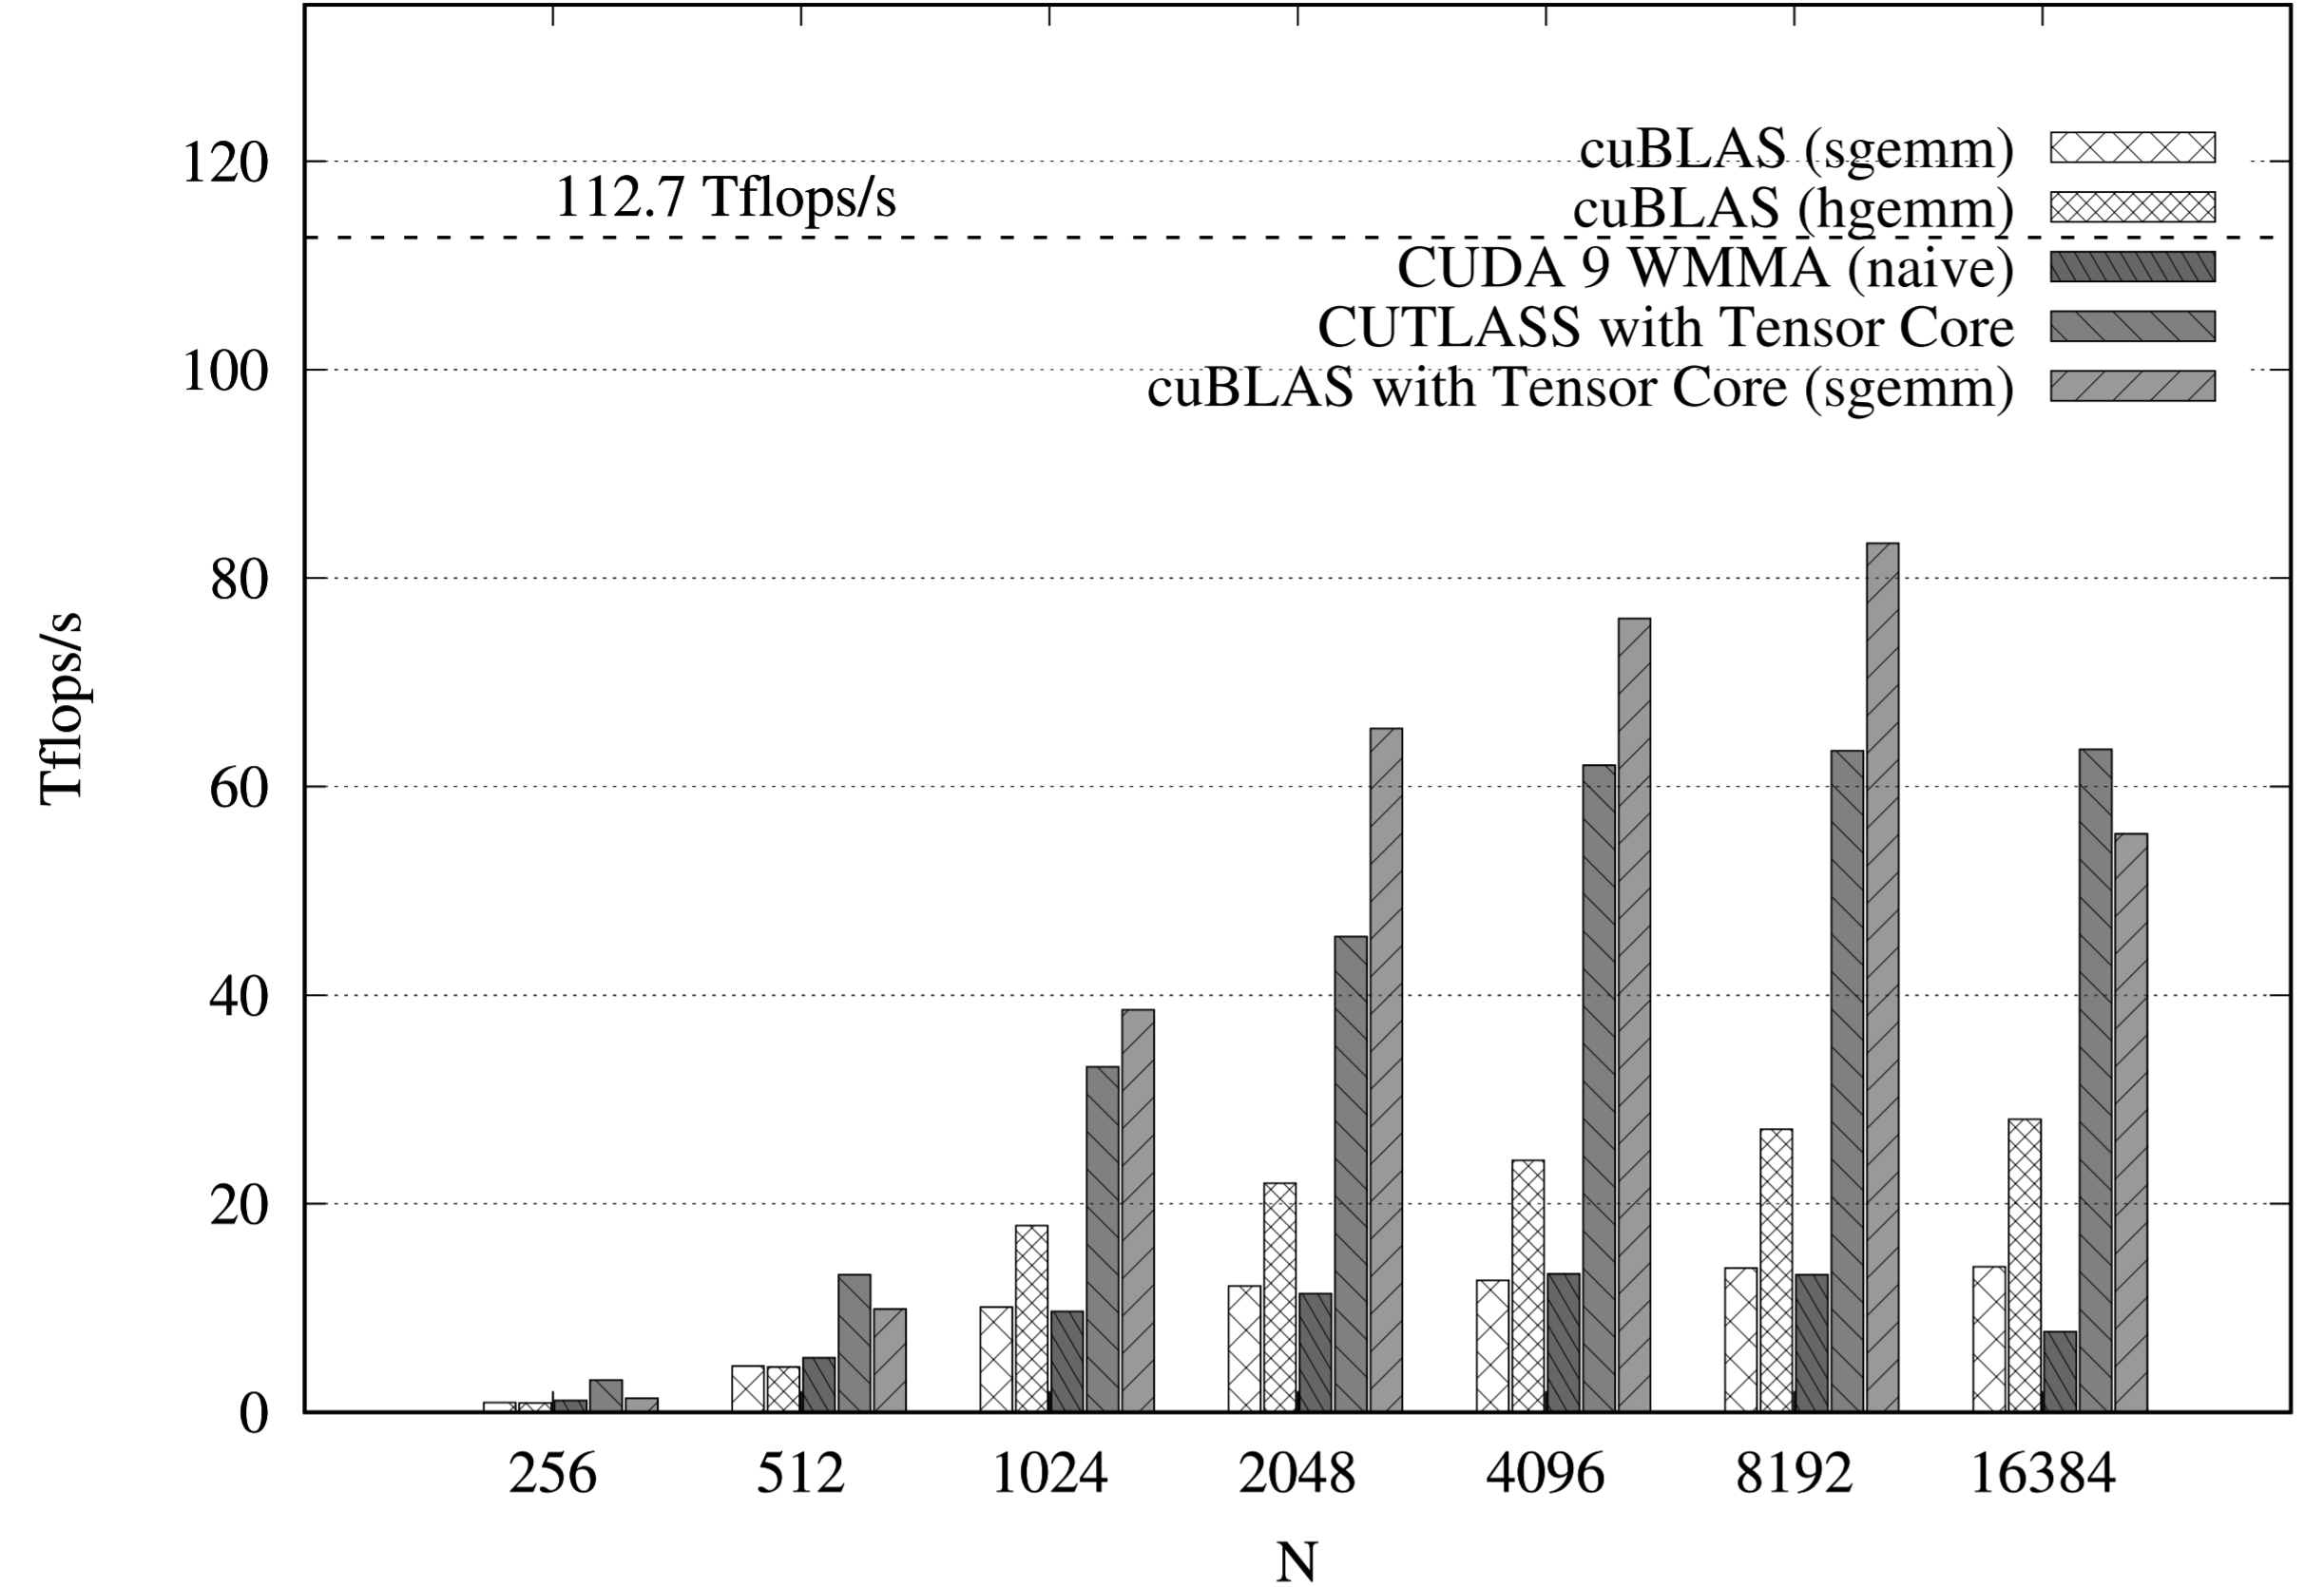
\includegraphics[width=7.5cm,height=5cm]{figures/ActualGemmPerf.jpg}
	\renewcommand{\thefigure}{\arabic{section}-\arabic{figure} }
	\renewcommand{\figurename}{图}
	\caption{官方白皮书给出的性能提升与实际测得性能提升\cite{VOLTAWHITEPAPER}\cite{TFCOMPARE}}
	\addtocounter{figure}{-1}
	\renewcommand{\thefigure}{\arabic{section}-\arabic{figure} }
	\renewcommand{\figurename}{Figure}
	\caption{Performance improvement in GEMM given by the official white paper and practical application\cite{VOLTAWHITEPAPER}\cite{TFCOMPARE}}
	\label{fig.PerfCompare}
\end{figure}
\par 在最近刚结束的GTC 2019会议中,NVIDIA发布了若干面向机器学习的硬件、软件。包括专为张量计算设计的Turing Tensor Core GPU,嵌入式平台的Jetson Nano\cite{JETSONNANO},将机器学习相关计算库整合的CUDA X\cite{CUDAX},这些都将在后文提到,但由于这些本质上都基于目前的Turing架构,故不会单独进行详细地说明。
\subsection{相关研究}
\par 本文的研究同时涉及硬件和软件:NVIDIA新架构的GPU与使用GPU加速计算的机器学习应用,注意这里的机器学习应用并不只是现在大行其道的深度学习,还包括传统的基于概率模型的方法等。
\par 在近年来深度学习迅猛发展之前,关于使用GPU并行化机器学习算法的研究就已有很多,甚至可以说正是基于GPU的强大并行计算能力,深度学习才能发展如此迅速。早在2005年,D. Steinkraus等人便对在GPU上实现机器学习算法进行了研究, 当时实现的算法是OCR,如今OCR能够非常快速、方便地通过各种框架、语言实现。然而这一研究奠定了使用GPU加速机器学习应用的基础\cite{GPUFORML}。之后的几年中,除去OCR外,基于GPU的各种并行机器学习算法包括kNN\cite{KNNG},支持向量机\cite{SMOSVM}都慢慢成熟。由于贝叶斯网络的精确推理是个NP难的问题,其性能受限于硬件水平,然而根据Md Vasimuddin等人的研究\cite{BAYESINF},通过并行方法将延迟降低了许多。由于传统机器学习方法有着延迟低、模型小、训练时间短、可解释性强等优点,在深度学习迅猛发展的今天,传统机器学习方法仍然占有很大的市场,故评估GPU对传统机器学习加速的性能是十分有必要的。本文中在评估传统机器学习的部分便采用了并行的支持向量机算法(SMO-SVM),如今,不管是在工业生产领域还是学术研究领域,该算法仍占有一席之地。
\par 之后不久,深度学习、神经网络便迎来了爆炸式的发展。实际上在二十世纪末,便已经有完整的神经网络算法的理论基础;在1979年,日本学者福岛邦彦提出了Neocognition模型,其中使用多层网络以及神经元对图像特征进行提取和筛选被认为是启发了卷积神经网络的开创性研究\cite{JAPANESSAY}。1989年,LeCun首次在论文中提出了“卷积”一次,卷积神经网络因此得名\cite{LENET}。在1993年,贝尔实验室对LeCun的工作进行了代码实现,并大量部署于手写支票识别系统,然而限于当时计算能力低下,基于神经网络的研究也停滞在了理论阶段,其主要原因便是网络中需要训练的参数太多,网络结构复杂,在当时没有芯片能满足如此高的性能要求\cite{NNML}。然而,随着高性能GPU芯片的出现,基于神经网络的方法正如日中天地发展。从TinyCNN等较轻量级、功能单一的库,到Tensor Flow、PyTorch、Caffe、Chain等完整、易于使用的框架,这些工具或是本身就是基于GPU编写的,或是慢慢更新对GPU的支持;目前市面上的绝大部分该类产品均支持使用GPU运行,单单使用CPU进行深度学习训练已经成为历史。在本文中,卷积神经网络由于它的广泛性、高性能、典型性,在本文中被选为深度学习部分评估的主要载体。
\par 而准确地对GPU以及机器学习的性能进行评估也尤为重要。且为了深入研究GPU对于机器学习应用的性能提升的幅度以及不同提升幅度的不同原因,单单是对训练时间进行统计、评估是不够的。因本文涉及NVIDIA新架构GPU中新加入的硬件以及对应CUDA中新加入的API等,故指令、运行流级别的分析是有必要的。Ali Bakhoda等人曾设计实现了一种在软件层面对CUDA执行流进行指令级别的模拟和仿真的系统GPGPU-SIM,该系统是基于Kepler架构的硬件以及CUDA 3.0版本,在缓存命中率、分支、指令乱序执行等方面能达到90-95\%与真实硬件的吻合程度\cite{GPGPUSIM}。在之后Mahmoud Khairy等人对该系统进行了改进,使其支持伏特架构(Volta)的GPU以及对应的CUDA 9.0 \cite{GPGPUSIM2}。然而,目前GPU硬件已经更新到图灵架构(Turing),基于安培架构(Ampere)的硬件也即将发布;对应的CUDA版本已经更新到了10.1,在指令执行、调度方式等方面都发生了很多的改变;且Mahmoud Khairy等人的工作主要着重于GPU的内存等方面。故能够准确评估新硬件的系统非常必要。本文中选用了nvprof、NSight等公开的工具,这些工具能从指令运行时间、访存、缓存命中率等方面对CUDA应用程序进行评估\cite{NSIGHT}。
\par 在新架构的GPU中,最为重要的便是新加入的计算单元:张量核心(Tensor Core),该运算单元能为深度神经网络中大量存在的张量计算带来明显的提升\cite{VOLTAWHITEPAPER},然而这些数据是NVIDIA官方白皮书中给出的数据,开发者社区中反映很少有情况能获得如NVIDIA官方宣传所能得到的性能提升;而关于Tensor Core的研究少之又少,故本文并非旨在填补这方面研究的空白,姑且在新的方向进行一些稚嫩的尝试;且由于在NVIDIA进行实习工作,有机会接触到许多内部资料,本文是一个很好的契机。
\par 当然,仅有理论计算性能的研究是无力的,最终本文还是会回归实际,使用实际应用中的模型,如各种结构的神经网络、广泛使用的支持向量机并行库对新架构的GPU进行评估。从广为各大厂商使用的深度学习性能评估工具DeepBench\cite{DEEPBENCH},到使用cuDNN从C++源码实现的卷积神经网络,再使用Tensor Flow框架实现的各种结构的网络,包括LeNet-5\cite{LENET},ResNet\cite{RESNET},MobileNet\cite{MOBILE}等,本文将由下而上对新架构硬件再浮点精度计算、张量计算、卷积计算、矩阵计算等方面进行评估,不求全面,只求能给出启发。

\subsection{我们的工作}
\par 近年来,深度学习与神经网络发展迅猛,为了应对日益提升的计算量要求,NVIDIA近年来持续、定期发布新架构GPU、嵌入式芯片以及对应的革新技术如张量核心、TensorRT、深度学习抗锯齿(DLSS)等,且重心逐渐从游戏业务向深度学习业务转移。
\par 同时,为了方便从业者搭建模型,各种框架层出不穷,考虑到计算量要求,这些框架陆续推出了GPU版本,对GPU硬件操作进行了抽象,然而对于硬件操作、细节的抽象使得框架无法完全利用硬件的性能,以及新硬件的特征,这也导致了理论性能与实际应用中的性能的巨大差距。
\par 为尽可能提升在实际应用场景中硬件性能的利用率,发掘新架构的提升潜力,本文将自底向上结合硬件特征对机器学习应用进行研究与评估,挖掘理论与实际不符的原因并提出适当的或是程序编写方面的,或是硬件架构方面的建议与展望。本文将主要从如下三个层面研究。
\begin{itemize}
	\item 基于性能评估的Benchmark,从指令、缓存、上下文切换等角度分析通用矩阵乘法、卷积运算在新架构GPU上的性能。
	\item 基于CUDA源码搭建深度学习和传统机器学习应用(卷积神经网络、支持向量机),分析较完整、涉及多种运算的应用在新架构GPU上的性能,并从纹理内存、调度方式上尝试优化。
	\item 基于深度学习框架Tensor Flow-GPU搭建完整的卷积神经网络,分析在贴近实际开发情况下,新架构GPU所能带来的性能提升。除训练过程外,网络推理过程也在研究范围内。最后,结合基于Benchmark,CUDA源码的实验结果,从纹理内存、数据精度、超参数等方面对网络训练过程进行优化。并利用TensorRT与相应硬件平台Jetson对网络推理过程进行优化。
\end{itemize}

\subsection{本文的组织结构}
\par 本文在第2章中介绍了该研究的背景和相关技术。首先介绍了NVIDIA GPU的硬件结构以及底层硬件的机制,由此引出伏特架构与图灵架构在硬件方面的创新与不同。之后自底向上介绍了NVIDIA GPU编程相关的软件。除神经网络训练外,本次实验还涉及神经网络推理,故对NVIDIA发布的神经网络推理优化工具以及相应硬件平台进行了简要介绍。最后列出了本次实验中使用的性能评估(Profiling)工具以及相应特征、应用场合。
\par 本文在第3章首先简要介绍实验平台以及相关工具。接着详细介绍了实验过程,包括多种基于性能测试的Benchmark(如矩阵乘加、卷积等)、基于CUDA源码的机器学习应用(包括深度学习应用与传统机器学习应用),除训练过程外,还对神经网络的推理、部署过程进行了评估和基于TensorRT的优化。最后针对完整的深度学习框架(Tensor Flow-GPU)的神经网络应用对训练和推理过程进行了评估。这一章中详细说明了实验结果以及相应的分析。在每个实验的最后给出了在程序编写、硬件结构方面的建议、展望。
\par 本文最后在第4章进行总结,并给出之后改进、展望与深入工作的设想、预期。

